\documentclass[12pt, twoside]{article}
\usepackage[francais]{babel}
\usepackage[T1]{fontenc}
\usepackage[latin1]{inputenc}
\usepackage[left=7mm, right=7mm, top=7mm, bottom=7mm]{geometry}
\usepackage{float}
\usepackage{graphicx}
\usepackage{array}
\usepackage{multirow}
\usepackage{amsmath,amssymb,mathrsfs}
\usepackage{soul}
\usepackage{textcomp}
\usepackage{eurosym}
 \usepackage{variations}
\usepackage{tabvar}


\pagestyle{empty}

\begin{document}

\section*{\center{Correction devoir maison 1}}


\bigskip


\ul{Exercice 1}: 

\begin{center} 
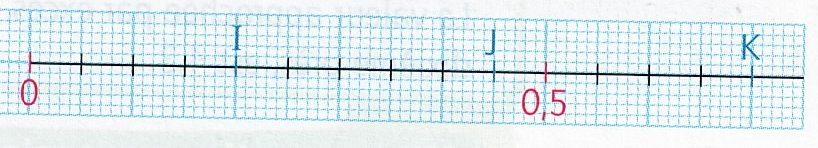
\includegraphics[width=11cm]{images/droite.jpg}
\end{center}


\bigskip

\ul{Exercice 2}: 


\begin{enumerate}
  \item 162 > 150 > 120 > 118 > 108
  \item  5,01 < 5,16 < 6,09 < 6,12 < 7,05
\end{enumerate}


\bigskip

\ul{Exercice 4}: 


\enskip

\begin{tabular}{|c|c|c|c|}
\hline

\begin{minipage}{4,5cm}
\qquad


Lecture

\qquad

\end{minipage}
&
\begin{minipage}{4cm}

\qquad


Fraction d�cimale


\qquad 
\end{minipage}
&
\begin{minipage}{4,5cm}

\qquad 


Somme d'un entier et de fractions d�cimales


\qquad 
\end{minipage}
&
\begin{minipage}{4cm}
\qquad 


Ecriture d�cimale

\qquad
\end{minipage} \\
\hline

\begin{minipage}{4,5cm}

\quad



\quad


423 unit�s et 5 dixi�mes

\quad

\quad

\end{minipage}
& 
$\dfrac{4235}{10}$ & 423 +  $\dfrac{5}{10}$ & 423,5  \\


\hline



0 unit� et 6 dixi�mes & $\dfrac{6}{10}$ ou $\dfrac{60}{100}$ & $0 +
\dfrac{6}{10}$ &

\begin{minipage}{4cm}
\quad


\quad


\begin{center}
0,60 
\end{center}

\quad

\quad
\end{minipage}
 \\


\hline


0 unit� et 9 centi�mes & 

\begin{minipage}{4cm}

\quad

\begin{center}
$\dfrac{9}{100}$
\end{center}
 

\quad
\end{minipage}


& 

$0+ \dfrac{9}{100}$  & 0,09 \\

\hline



11 unit�s et 4 milli�mes & $\dfrac{11004}{1000}$ 

& 

\begin{minipage}{4,5cm}

\qquad

\begin{center}
$11+ \dfrac{4}{1000}$ 
\end{center}


\qquad
\end{minipage}


& 

11,004 \\

\hline

\begin{minipage}{4,5cm}

\quad



\quad


38 unit�s et 23 centi�mes

\quad

\quad

\end{minipage} 

& 
$\dfrac{3823}{100}$ 

& 

$38+\dfrac{23}{100}$


& 

38,23 \\

\hline

\end{tabular}



\bigskip


\bigskip

\ul{Exercice 5}: 

\enskip

\begin{center}
\begin{tabular}{|c|c|c|}

\hline

\quad & 
\begin{minipage}{5cm}

\quad


valeur approch�e par d�faut de 9,354

\quad
\end{minipage}
&
\begin{minipage}{5cm}

\quad


valeur approch�e par exc�s de 9,354

\quad
\end{minipage} \\

\hline

\begin{minipage}{5cm}
\quad

� l'unit� pr�s

\quad
\end{minipage}
&

9

&

10 \\

\hline

\begin{minipage}{5cm}
\quad

au dixi�me pr�s

\quad
\end{minipage}
&

9,3

&

9,4 \\


\hline
\end{tabular}
\end{center}
\end{document}
